\documentclass[a4paper]{article}
\usepackage{fancyhdr}
\usepackage[left=2cm,right=1.5cm,top=1.5cm,bottom=1cm,includeheadfoot]{geometry}
\usepackage{listings}
\usepackage{graphicx}
\usepackage{amsmath}

\title{ROBOTICS Series 6}
\author{Fabienne Guertler 12-935-508}

\pagestyle{fancy}
\makeatletter
\let\runauthor\@author
\let\runtitle\@title
\makeatother
\lhead{\runtitle}
\rhead{\runauthor}

\renewcommand\thesection{\arabic{section}}
\renewcommand\thesubsection{\thesection.\alph{subsection}}

\begin{document}
	\section{Colors}
		\subsection{Calibration script}
			For this exercise we used the measurements from the previous series. But this time 				we included a evaluation of our results in percentage to help us find an algorithm
			to recognize colors.
			
			\begin{figure}[h!]
				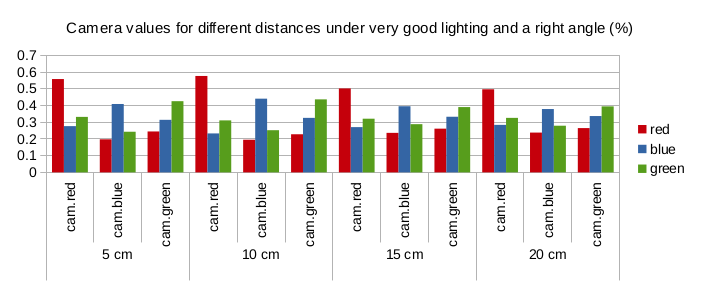
\includegraphics[width=\linewidth]{CamValuesPerc.png}
				\caption{Color measurements in percentage}
			\end{figure}						
			
			\noindent We used this analysis to come up with the following ranges for the 
			colors:
								
			\begin{table}[h!]
				\begin{center}
				\begin{tabular}{c||c|c|c}
					& cam.red & cam.blue & cam.green\\
					\hline
					\hline
					Red & 50\% - 60\% & 15\% - 25\% & 20\% - 30\% \\
					Blue & 20\% - 30\% & 35\% - 45\% & 30\% - 35\% \\
					Green & 30\% - 35\% & 20\% - 30\% & 35\% - 45\% \\ 
				\end{tabular}
				\caption{Color ranges in percentage}
				\label{tab:ColorRanges}
				\end{center}	
			\end{table}
			
			\noindent From the values of Table \ref{tab:ColorRanges} we figured out algorithms 
			to recognize colors. For example, the ratio of red is generally 2 to 4 times bigger 
			than the ratio of blue.	
			\begin{align*}
				2 \cdot cam.blue \leq &cam.red \leq 4 \cdot cam.blue \\
				2 \cdot cam.green \leq &cam.red \leq 3 \cdot cam.green\\
			\end{align*}
			Similarly you can find a calculation for green and blue.
			\begin{align*}
				14 \cdot cam.red \leq 12 \cdot &cam.blue \leq 27 \cdot cam.red \\
				7 \cdot cam.green \leq 7 \cdot &cam.blue \leq 9 \cdot cam.green\\
				\\
				14 \cdot cam.red \leq 12 \cdot &cam.green \leq 27 \cdot cam.red \\
				7 \cdot cam.green \leq 7 \cdot &cam.green \leq 9 \cdot cam.green\\
			\end{align*}	
			\newpage
			
			\textit
			{
				for i in 0:4 do\\  \indent \indent camRed += cam.red[i+28]\\ \indent end\\ 
				\indent camRed /= 4\\
			}			
				
			\noindent We took 5 pixels in the middle of the camera and calculated the average, 
			unlike last time where we calculated the average of every tenth pixels over all the 
			pixels. We used this approach because we felt that when driving around, the pixel 
			right in the front are most important. With this calculation the e-puck's color 
			cognition is similar to a human's in the fact that we also mostly see what is right 
			in front of us and only very little of what is on the sides. Well, like this the e-
			puck does not recognize any colors on the sides at all. This could be a further 
			improvement of the color recognition algorithm. One could try to find a calculation 
			where the pixels on the front are weighted the most and those on the sides are 
			weighted less. Unfortunately we did not get to this step.\\
			
			\noindent The code that we used to determine the color and the subsequent behavior is 
			not quite like the calculation we came up with in theory but close. As most of the 
			time, when trying to apply theory to the real implementation for the e-puck, we had to 
			adjust some bounds to get a good result.\\
			
			\textit
			{
				if 7*camRed $\leq$ 6*(camBlue+b) and 4*(camBlue-b) $\leq$ 9*camRed and\\
	   \indent \indent camGreen-b $\leq$ camBlue then\\
		\indent \indent \indent color = BLUE\\ \indent [...]\\ \indent end\\			
			}
			
			\noindent Here, for the calculation of the color blue we deleted one upper bound and 
			used a variable b to adjust. Compared to our calculations of the last series the color 
			recognition worked significantly better.
			 
		\newpage							
		\subsection{Approach color}
		\noindent We chose \textit{RED} as the color to approach. Our idea for this exercise was 
		for the e-puck to change behavior according to which	color he sees. So in our case, 
		whenever the e-puck recognizes the color \textit{RED} he switches to the \textit{LOVE} 
		behavior. We implemented this as described in Breitenberg's "Vehicules - Experiments in 
		Synthetic Psychology".\\ 
		
		\textit
		{
			if color ==  NO\_COLOR  then\\ \indent \indent leds[4] = 0\\ \indent \indent leds[2] = 
			0\\ \indent \indent leds[6] = 0\\ \indent \indent behavior = EXPLORER\\ \\ \indent
			elseif color == RED then\\ \indent \indent leds[4] = 1 [...]\\ \indent \indent
			behavior = LOVE\\
		}
		
		\noindent It always checks the behavior and calls the corresponding subroutine. This 
		approach worked quite good but it needs a good color recognition. If for example the color 
		recognition flickers, the behavior flickers as well. The e-puck also does not actually 
		follow the color. As long as the e-puck sees \textit{RED} he acts as a \textit{LOVER} 
		which results in him following the object. But the \textit{LOVE} behavior does not care 
		about color it works with proximities as seen in series 3. For us this was the 
		implementation with the best results.\\
		
\end{document}